% ============================ Part 4: Supervised fine-tuning ============================
\section{Part 4 $\cdot$ SFT}
\partslide{4}{Supervised fine-tuning}{following instructions}

\begin{frame}{Pretrain once, fine-tune many times}
\begin{columns}[c]
\begin{column}{0.5\textwidth}
\begin{itemize}\setlength{\itemsep}{6pt}
  \item \textbf{Pretraining} is done \emc{once}, by a few labs: trillions of tokens, months of compute, tens of millions of dollars.
  \item \textbf{Fine-tuning} \emc{continues training the same network} on a small, targeted dataset. Hours on one GPU.
  \item The pretrained weights $\theta_0$ are the starting point. Fine-tuning moves them a little and keeps what pretraining learned.
  \item The fine-tuning we care about today is \textbf{instruction tuning}: turning the text continuer into an assistant.
\end{itemize}
\end{column}
\begin{column}{0.48\textwidth}
\centering
\begin{tikzpicture}[font=\small,>=Latex,node distance=5mm,
  box/.style={draw,rounded corners,minimum width=3.3cm,align=center},
  note/.style={text width=2.7cm,font=\footnotesize,text=uvanavy!80!black,align=left}]
  \node[box,fill=uvablue!12,minimum height=1cm] (pre) {\textbf{pretraining}\\web text, $10^{13}$ tokens};
  \node[box,fill=softgray,below=of pre] (th0) {pretrained weights $\theta_0$};
  \node[box,fill=okgreen!12,below=of th0,minimum height=1cm] (ft) {\textbf{fine-tuning}\\$10^4$--$10^6$ examples};
  \node[box,fill=softgray,below=of ft] (th) {fine-tuned weights $\theta$};
  \draw[->,thick] (pre) -- (th0); \draw[->,thick] (th0) -- (ft); \draw[->,thick] (ft) -- (th);
  \node[note,right=3mm of th0] {same architecture,\\same softmax head,\\same loss function};
  \node[note,right=3mm of ft] {small learning rate,\\a few epochs};
\end{tikzpicture}
\end{column}
\end{columns}
\end{frame}

\begin{frame}{Instruction tuning: the data}
\begin{columns}[T]
\begin{column}{0.5\textwidth}
\textbf{Instruction--response pairs} written or curated by people:
\begin{userbox}Label the sentiment of this sentence: \emph{The movie wasn't that great.}\end{userbox}
\begin{modelbox}negative\end{modelbox}
\begin{userbox}Translate to Spanish: \emph{The office was built in three months.}\end{userbox}
\begin{modelbox}La oficina se construy\'o en tres meses.\end{modelbox}
\end{column}
\begin{column}{0.48\textwidth}
\textbf{Chat format:} multi-turn, with roles, serialized with special tokens:
\begin{tcolorbox}[colback=softgray,colframe=softgray!60!black,boxrule=0.4pt,arc=3pt,left=5pt,right=5pt,top=3pt,bottom=3pt,fontupper=\scriptsize\ttfamily]
\{"role": "user", "content": "Weather today?"\}\\
\{"role": "assistant", "content": "Sunny, high of 75."\}\\
\{"role": "user", "content": "And tomorrow?"\}\\
\{"role": "assistant", "content": "Partly cloudy, 72."\}
\end{tcolorbox}
\begin{itemize}\setlength{\itemsep}{3pt}
  \item The model learns when to \emc{start} (right after the \texttt{<assistant>} marker), when to \emc{stop} (by emitting \texttt{<eos>}), and to follow the instruction.
  \item $10^4$--$10^6$ examples, tiny next to $10^{13}$ pretraining tokens.
\end{itemize}
\end{column}
\end{columns}
\end{frame}

\begin{frame}{Where instruction data comes from}
\begin{columns}[T]
\begin{column}{0.5\textwidth}
\centering
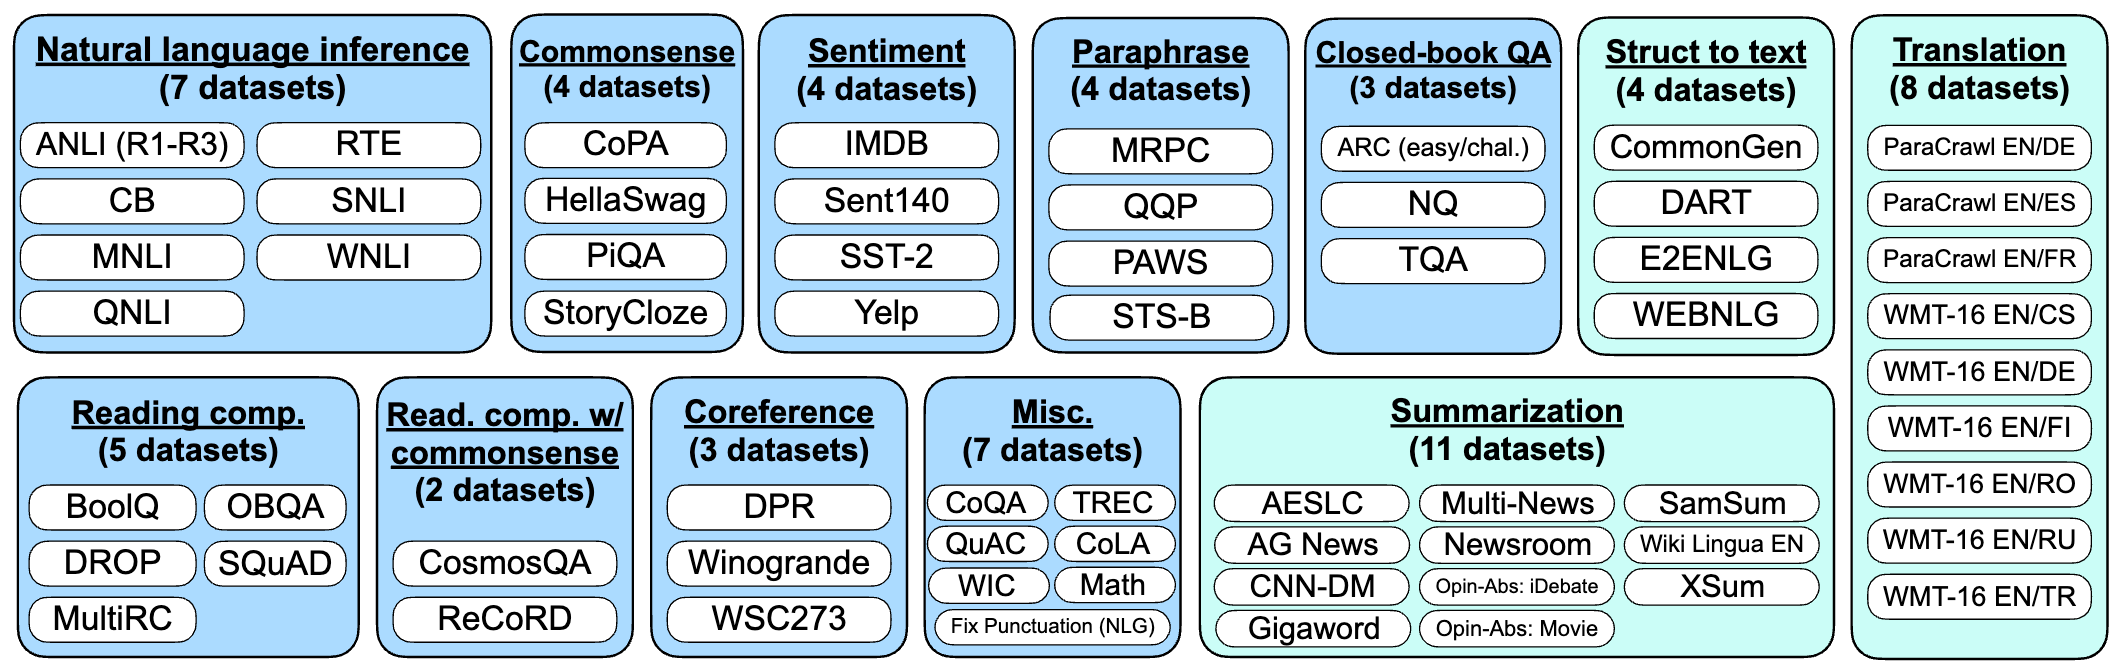
\includegraphics[width=\textwidth]{figs/flan_collection.png}\\[2pt]
\scriptsize \textbf{FLAN} (\href{https://arxiv.org/abs/2109.01652}{Wei et al., 2022}): 62 existing NLP datasets in 12 task clusters, each rephrased as natural-language instructions.
\end{column}
\begin{column}{0.48\textwidth}
\centering
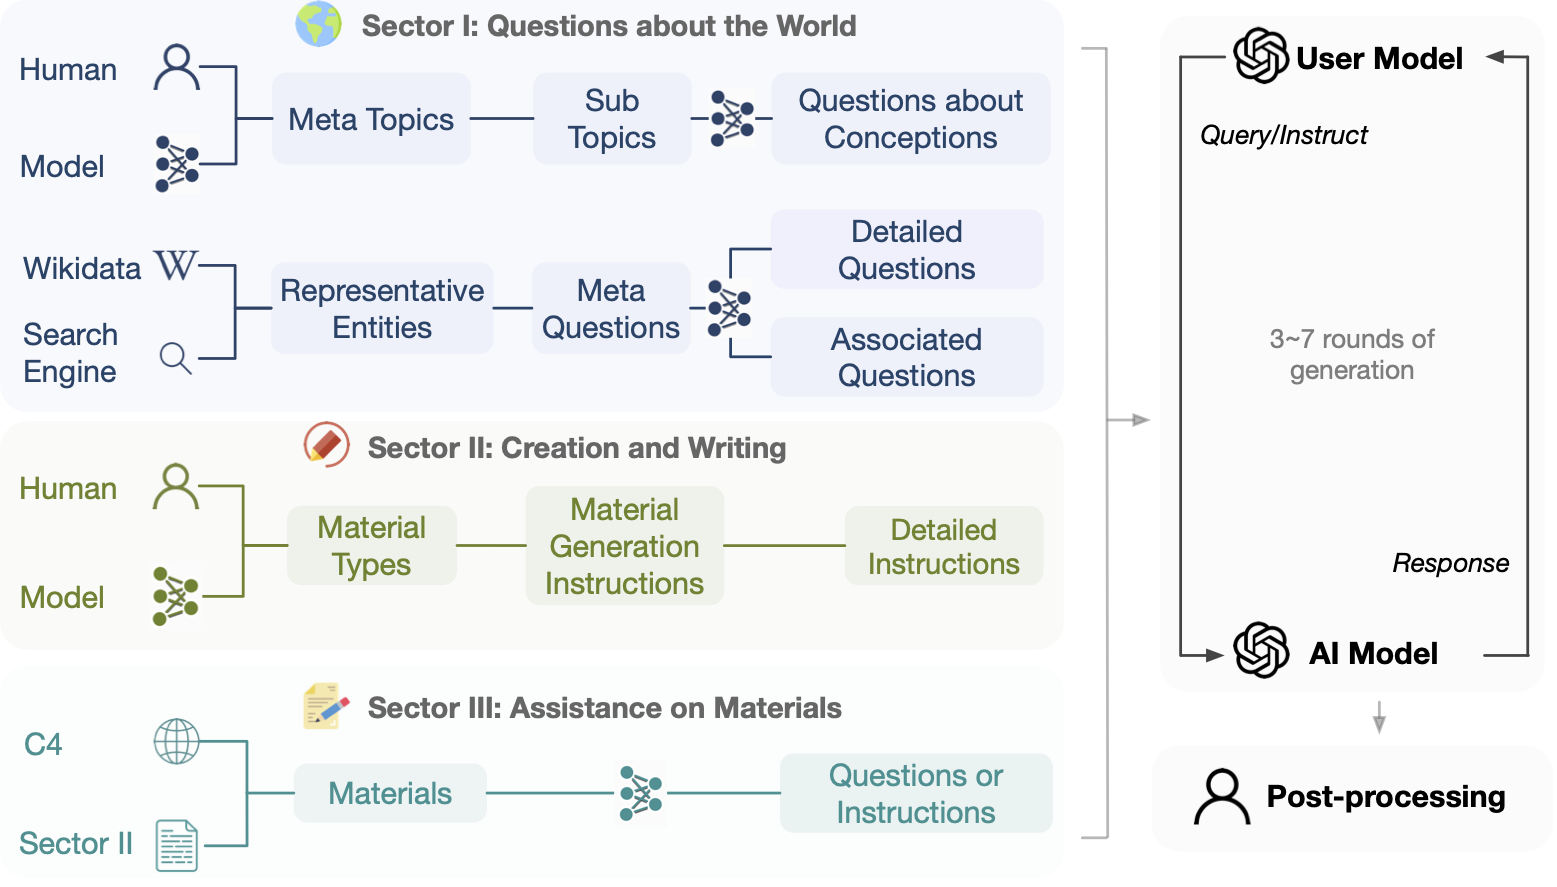
\includegraphics[width=\textwidth]{figs/ultrachat.png}\\[2pt]
\scriptsize \textbf{UltraChat} (\href{https://arxiv.org/abs/2305.14233}{Ding et al., 2023}): millions of multi-turn dialogues generated by having one LLM play the user and another the assistant.
\end{column}
\end{columns}
\vspace{6pt}
\begin{itemize}\setlength{\itemsep}{3pt}
  \item \textbf{Diversity} of tasks and phrasings matters more than the number of examples.
  \item Today much of the data is synthetic: strong models write the demonstrations, humans filter.
\end{itemize}
\end{frame}

\begin{frame}{SFT loss: the same cross-entropy, on the response tokens}
\textbf{Supervised fine-tuning (SFT) objective} on pairs $(x, y)$ = (prompt, response):
\[
  \mathcal{L}_{\text{SFT}}(\theta) = -\sum_{(x,y)\in\mathcal{D}} \sum_{t=1}^{|y|} \log p_\theta\big(y_t \mid x, y_{<t}\big)
\]
\begin{center}
\begin{tikzpicture}[font=\scriptsize,>=Latex]
  \foreach \i/\w in {1/{\texttt{<user>}},2/{Say},3/{hello},4/{in},5/{Spanish},6/{\texttt{<assistant>}}}{
    \node[draw,fill=softgray,rounded corners,minimum height=0.5cm,inner sep=3pt] (a\i) at (1.5*\i-1.5,0) {\w};
  }
  \foreach \i/\w in {1/hola,2/\texttt{<eos>}}{
    \node[draw,fill=okgreen!20,rounded corners,minimum height=0.5cm,inner sep=3pt] (b\i) at (1.5*\i+7.5,0) {\w};
  }
  \draw[decorate,decoration={brace,amplitude=4pt,mirror},gray] (a1.south west) -- (a6.south east) node[midway,below=5pt,text=midgray] {prompt $x$: context only, no loss, no gradient};
  \draw[decorate,decoration={brace,amplitude=4pt,mirror},okgreen!70!black] (b1.south west) -- (b2.south east) node[midway,below=5pt,text=okgreen!70!black] {response $y$: loss on each token};
  \draw[->,okgreen!70!black,thick] (a6.north) to[bend left=30] node[above,xshift=-6mm] {$-\log p_\theta(\text{hola}\mid x)$} (b1.north);
  \draw[->,okgreen!70!black,thick] (b1.north) to[bend left=70] node[above,xshift=4mm] {$-\log p_\theta(\texttt{<eos>}\mid x,\text{hola})$} (b2.north);
\end{tikzpicture}
\end{center}
\vspace{-4pt}
\begin{itemize}\setlength{\itemsep}{4pt}
  \item Identical to the pretraining loss, except prompt tokens are \textbf{context only} (``loss masking'').
  \item Same network, same softmax head, same optimizer. Maximizing the likelihood of the demonstrations = learning to \textbf{imitate} the demonstrated behavior (``behavior cloning'' in RL terms).
\end{itemize}
\keybox{\textbf{Nothing new in the math, only new data.} What it learns: the \emc{format and behavior} of an assistant.}
\end{frame}

\begin{frame}{What instruction tuning gives you: zero-shot generalization}
\begin{columns}[T]
\begin{column}{0.46\textwidth}
\centering
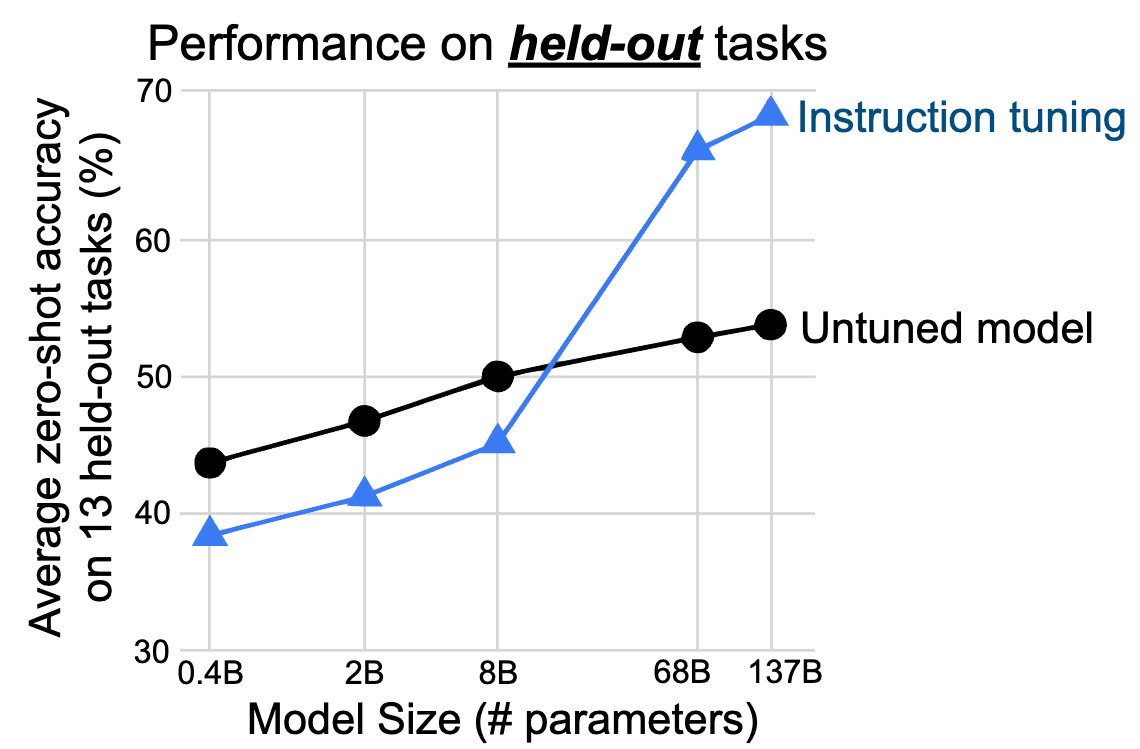
\includegraphics[width=0.95\textwidth]{figs/flan_scale.png}\\[2pt]
\scriptsize Zero-shot accuracy on \emph{held-out} task types vs.\ model size (FLAN, \href{https://arxiv.org/abs/2109.01652}{Wei et al., 2022}).
\end{column}
\begin{column}{0.52\textwidth}
\centering
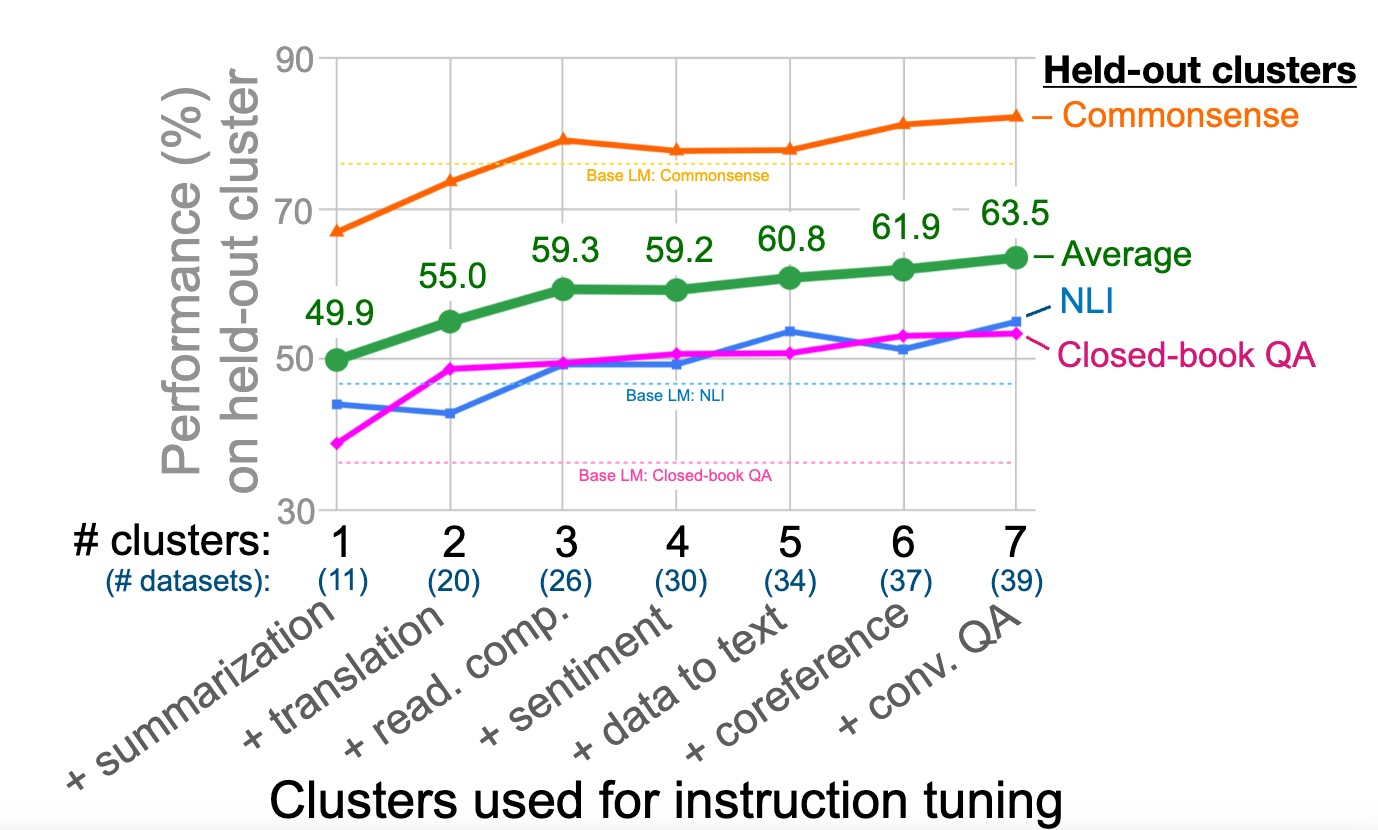
\includegraphics[width=0.95\textwidth]{figs/flan_clusters.png}\\[2pt]
\scriptsize More task clusters in the fine-tuning mix $\Rightarrow$ better on unseen clusters.
\end{column}
\end{columns}
\vspace{6pt}
\begin{itemize}\setlength{\itemsep}{4pt}
  \item Train on 60 tasks phrased as instructions $\Rightarrow$ the model follows \textbf{new} instructions with no examples in the prompt.
  \item Chat-style data does the same for conversation: this is how a text continuer becomes a chatbot.
\end{itemize}
\end{frame}

\begin{frame}{The limits of imitation}
SFT = imitate human-written responses. Four problems:
\begin{enumerate}\setlength{\itemsep}{8pt}
  \item \textbf{Costly supervision:} someone must \emph{write} a full, high-quality response for every prompt.
  \item \textbf{Every token counts the same:} the loss penalizes a typo exactly like a factual error.
  \item \textbf{A ceiling:} the model can only copy the demonstrator, and for open-ended tasks there is no single ``right'' answer.
  \item \textbf{Judging is easier than writing:} it is far easier to say \emph{which of two answers is better}, or whether an answer is \emph{correct}, than to write the best answer.
\end{enumerate}
\end{frame}

\begin{frame}{A new paradigm: learn from evaluation, not demonstration}
\begin{center}
\begin{tikzpicture}[font=\small,>=Latex,node distance=8mm]
  \node[draw,rounded corners,fill=okgreen!12,minimum width=3.4cm,minimum height=1cm,align=center] (sft) {\textbf{SFT}\\\scriptsize copy a human response};
  \node[draw,rounded corners,fill=uvaorange!15,minimum width=3.4cm,minimum height=1cm,align=center,right=2.6cm of sft] (rl) {\textbf{RL}\\\scriptsize generate $\to$ score $\to$ update};
  \node[below=4mm of sft,align=center,font=\scriptsize,text=midgray] {needs: a written answer per prompt};
  \node[below=4mm of rl,align=center,font=\scriptsize,text=midgray] {needs: a \emph{score} per generated answer};
  \draw[->,very thick,uvanavy] (sft) -- node[above,font=\scriptsize] {the rest of today} (rl);
\end{tikzpicture}
\end{center}
\vspace{4pt}
\keybox{Let the model \emc{generate} its own responses, \emc{score} them, and update toward the ones that scored well. That is \textbf{reinforcement learning}.}
\vspace{6pt}
Two kinds of score:
\begin{itemize}\setlength{\itemsep}{3pt}
  \item \textbf{Human preference:} ``A is better than B'' $\to$ a learned reward model (RLHF), or used directly (DPO).
  \item \textbf{Correctness:} ``the answer is right'' $\to$ a program that checks it (RLVR, GRPO).
\end{itemize}
\end{frame}
